\documentclass{beamer}

\mode<presentation> {
\usetheme{Madrid}
}

\usepackage{graphicx}
\usepackage{svg}
\usepackage{booktabs}
\usepackage{amsmath}
\usepackage[french]{babel}
\usepackage{url,color}
\usepackage{subfigure}
\usepackage{amsthm,amsfonts,amssymb,amscd,amsxtra, multicol}
\usepackage{comment}

\graphicspath{ {./images/} }

% \setbeamertemplate{caption}[numbered]
% \newcommand{\tabitem}{~~\llap{\textbullet}~~}

\title{Conception d'un SaaS pour les cours en ligne en milieu universitaire}
\author[Hans TOGNON]{Hans B. K. \textbf{TOGNON} \\ Supervisé par Ing. Miranda \textbf{GNONLONFOUN}}
\institute[IFRI]{
\textbf{I}nstitut de \textbf{F}ormation et de \textbf{R}echerche en  \textbf{I}nformatique \\
\medskip
% \textbf{\color{magenta}\href{mailto:contact@ifri.uac.bj}{contact@ifri.uac.bj}}
}

\begin{document}
% %%%%%%%%%%%%%%%%%%%%%%%%%%%%%%%%%%
% Title Page
% %%%%%%%%%%%%%%%%%%%%%%%%%%%%%%%%%%
\begin{frame}
  \thispagestyle{empty}
  \begin{multicols}{2}
    \begin{figure}
        \flushleft
        
\includegraphics[width=0.11\textwidth]{logoifri}
    \end{figure}
    \begin{figure}
        \flushright
        
\includegraphics[width=0.1\textwidth]{logouac}
    \end{figure}
    \end{multicols}
    \vspace{-1cm}
  \titlepage
  \end{frame}

% %%%%%%%%%%%%%%%%%%%%%%%%%%%%%%%%%%
% ToC
% %%%%%%%%%%%%%%%%%%%%%%%%%%%%%%%%%%
\begin{frame}
  \frametitle{PLAN}
  \begin{itemize}
    \item Introduction
    \item Revue de Littérature
    \item Matériels et méthodes
    \item Prototype
    \item Discussion \& Perspectives
    \item Conclusion
  \end{itemize}
\end{frame}

% %%%%%%%%%%%%%%%%%%%%%%%%%%%%%%%%%%
% Introduction
% %%%%%%%%%%%%%%%%%%%%%%%%%%%%%%%%%%
\begin{frame}
  \begin{center}
    \section{\huge{Introduction}}
  \end{center}
\end{frame}

\begin{frame}{Introduction : \small{Contexte}}
  Les méthodes d'enseignement évoluent avec l'utilisation croissante 
  du numérique pour une éducation plus créative et collaborative, y 
  compris dans l'enseignement supérieur, notamment en réponse aux défis 
  tels que la pandémie de COVID-19 et l'indisponibilité de cadres de cours 
  adéquats.
\end{frame}

\begin{frame}{Introduction : \small{Problématique}}
  L'expansion des cours en ligne nécessite une organisation logistique 
  accrue et un investissement financier. Les solutions génériques s'avèrent dans bien 
  des cas inadequates ou coûteuses.
\end{frame}


\begin{frame}
  \frametitle{Introduction : \small{Objectifs}}
    Concevoir un prototype d'application permettant la tenue de cours en ligne.
\end{frame}

\begin{frame}
  \frametitle{Introduction : \small{Objectifs} - \footnotesize{Fonctionnalités}}
  \begin{itemize}
    \item Organiser les classes des entités en sections bien définies ;
    \item Définir l'organisation temporelle des classes ;
    \item Organiser des sessions d’audio-conférence ;
\end{itemize}
\end{frame}

\begin{frame}
  \frametitle{Introduction : \small{Objectifs} - \footnotesize{Fonctionnalités}}
  \begin{itemize}
    \item Emuler, un tant soit peu, un environnement de classe présentiel via les fonctionnalités intégrées ;
    \item Minimiser les coûts requis dans le cadre de la mise en oeuvre d’une solution de classe virtuelle.
\end{itemize}
\end{frame}

% %%%%%%%%%%%%%%%%%%%%%%%%%%%%%%%%%%
% Revue de Littérature
% %%%%%%%%%%%%%%%%%%%%%%%%%%%%%%%%%%
\begin{frame}
  \begin{center}
    \section{\huge{Revue de Littérature}}
  \end{center}
\end{frame}

\begin{frame}{Revue de Littérature : \small{Formation à distance}}
  La formation à distance est une forme d’enseignement ou l’enseignant et l’étudiant sont séparés dans le temps et/ou par l’espace. 
\end{frame}

\begin{frame}{Revue de Littérature : \small{Formation à distance}}
  Les débuts remontent à 1728 avec 
  Caleb Phillips qui enseignait la sténographie par correspondance, 
  et Isaac Pitman est considéré comme le créateur du premier cours 
  d'enseignement à distance moderne.
\end{frame}

\begin{frame}{Revue de Littérature : \small{Formation à distance}}
  L'avénement d'Internet ouvre la voie à plusieurs formes de cours :
  \begin{itemize}
    \item \textbf{MOOC}s: Massive Open Online Courses
    \item \textbf{SMOC}s: Synchronous Massive Online Courses
    \item \textbf{SPOC}s: Small Private Online Courses
    \item \textbf{SSOC}s: Synchronous Small Online Courses
  \end{itemize}
\end{frame}

\begin{frame}{Revue de Littérature : \small{Communication en temps réel}}
  Les outils de communications en temps réel désignent une catégorie de 
  logiciels qui garantissent le traitement et la transmission instantanée, 
  ou avec un délai fortement négligeable, de l’information.
\end{frame}

\begin{frame}{Revue de Littérature : \small{Communication en temps réel}}
  Parmi les protocoles 
  permettant ce type de communication, le plus en vogue reste \textbf{Web Real-Time Communication} (\textit{WebRTC}).
\end{frame}

\begin{frame}{Revue de Littérature : \small{ Software as a Service}}
  Un modèle de distribution logicielle ne nécéssitant aucune installation locale. L'application est accessible en ligne.
\end{frame}

\begin{frame}{Revue de Littérature : \small{Solutions existantes}}
  \begin{itemize}
    \item Google Classrooms / Google Meet
    \item Zoom
    \item Moodle / BigBlueButton
  \end{itemize}
\end{frame}

\begin{frame}{Revue de Littérature : \small{Limites}}
  \begin{itemize}
    \item Limite du nombre de participants
    \item Consommation large de la bande passante
    \item Investissement financier conséquent
    \item Complexité technique et/ou de prise en main
  \end{itemize}
\end{frame}
% %%%%%%%%%%%%%%%%%%%%%%%%%%%%%%%%%%
% Matériels et méthodes
% %%%%%%%%%%%%%%%%%%%%%%%%%%%%%%%%%%
\begin{frame}
  \begin{center}
    \section{\huge{Matériels et Méthodes}}
  \end{center}
\end{frame}

\begin{frame}{Matériels et Méthodes : \small{UML}}
  Une méthode de visualisation d’architecture logicielle permettant de modéliser l’architecture logicielle d’un système.
\end{frame}

\begin{frame}{Matériels et Méthodes : \small{UML} - \footnotesize{Diagramme de cas d'utilisation}}
  \begin{figure}[H]
    \centering
    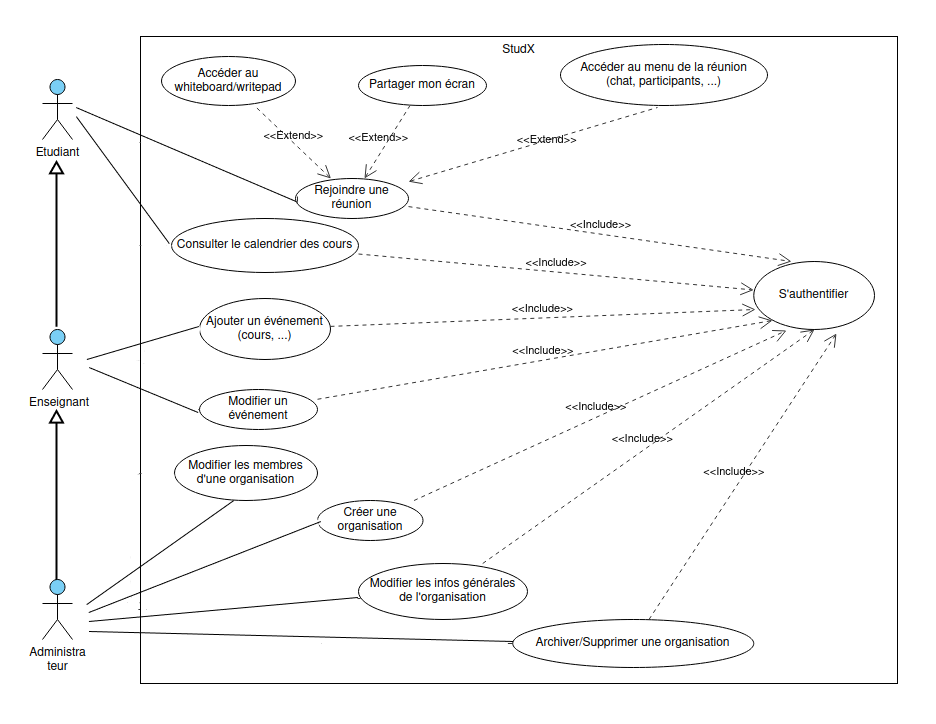
\includegraphics[width=\textwidth]{../../images/use-cases-diag.png}
    \caption{Cas d'utilisation}
\end{figure}

\end{frame}

\begin{frame}{Matériels et Méthodes : \small{UML} - \footnotesize{Diagramme de classe}}
  \begin{figure}[H]
    \centering
    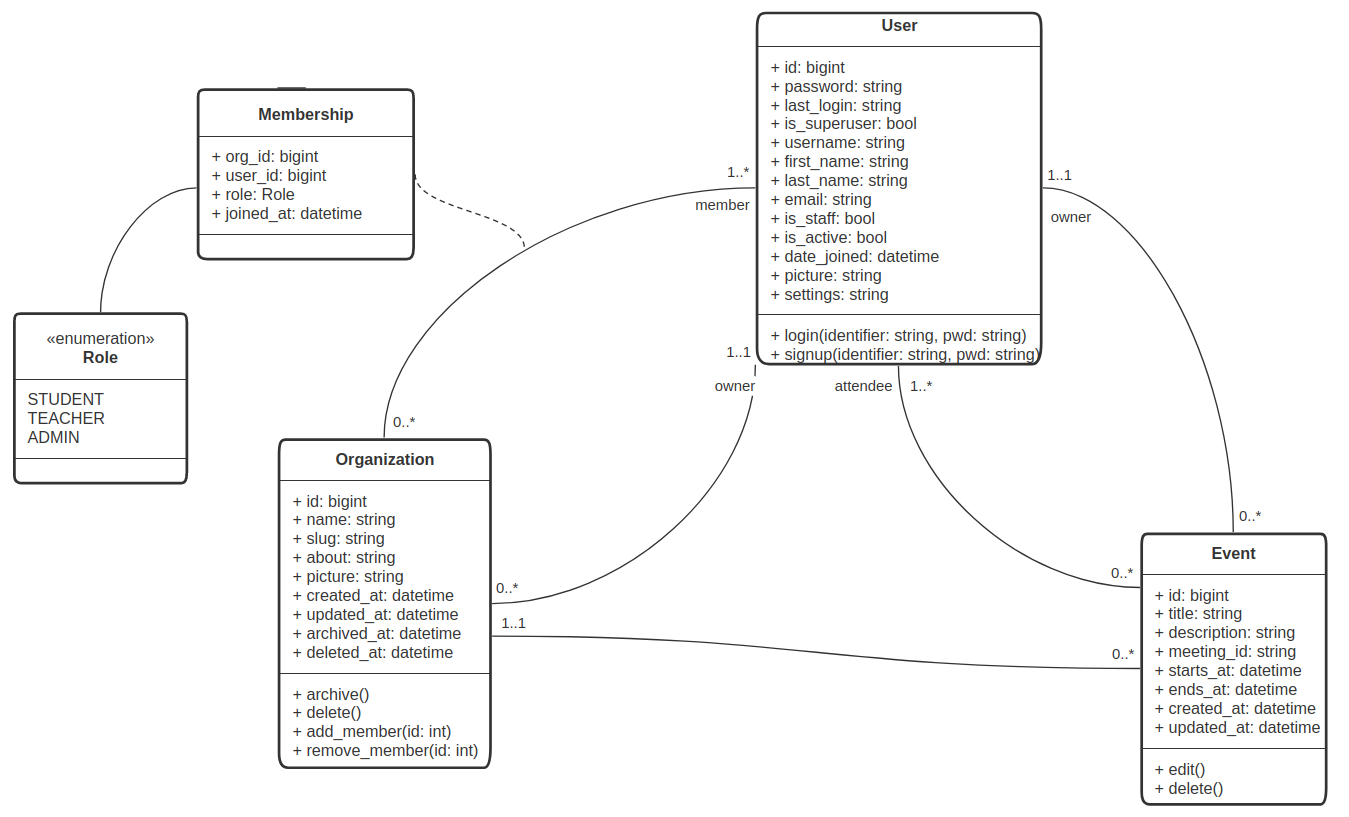
\includegraphics[width=\textwidth]{../../images/class-diag.png}
    \caption{Diagramme de classe}
\end{figure}
\end{frame}

\begin{frame}{Matériels et Méthodes : \small{UML} - \footnotesize{Diagramme de séquence}}
  \begin{figure}[H]
    \centering
    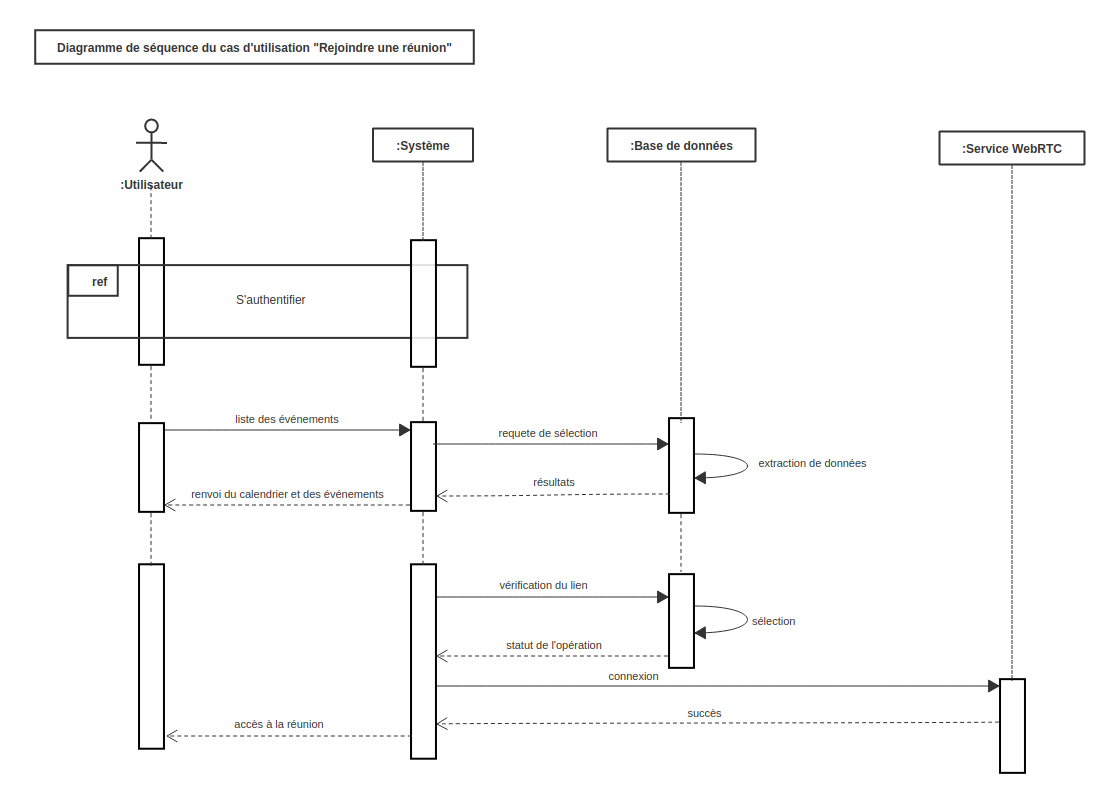
\includegraphics[width=0.9\textwidth]{../../images/join-meet-sequence-diag.png}
    \caption{Diagramme de séquence (fonctionnalité principale)}
\end{figure}
\end{frame}

\begin{frame}{Matériels et Méthodes : \small{Architecture Logicielle}}
  \begin{figure}[H]
    \centering
    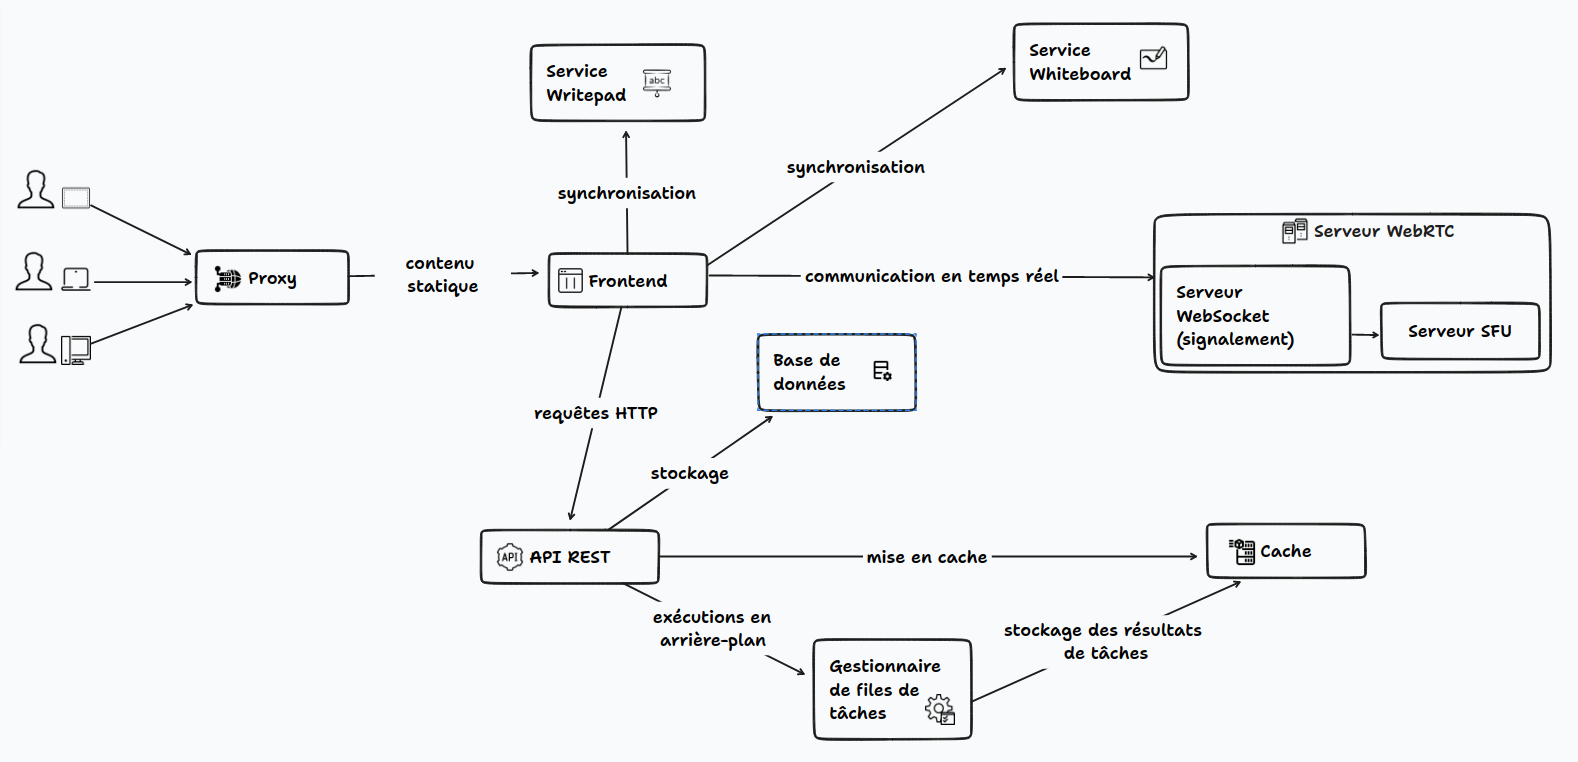
\includegraphics[width=1.05\textwidth]{../../images/studx-system-design.png}
    \caption{Architecture logicielle de \textbf{StudX}}
\end{figure}
\end{frame}

\begin{frame}{Matériels et Méthodes : \small{Technologies}}
  \begin{figure}[H]
    \centering
    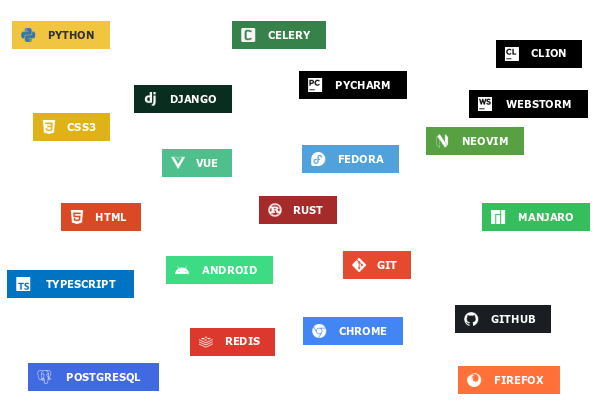
\includegraphics[width=0.9\textwidth]{tech-stack}
    \caption{Outils technologiques}
\end{figure}
\end{frame}

% %%%%%%%%%%%%%%%%%%%%%%%%%%%%%%%%%%
% Prototype
% %%%%%%%%%%%%%%%%%%%%%%%%%%%%%%%%%%
\begin{frame}
  \begin{center}
    \section{\huge{Prototype}}
  \end{center}
\end{frame}


% %%%%%%%%%%%%%%%%%%%%%%%%%%%%%%%%%%
% Résultats et Perspectives
% %%%%%%%%%%%%%%%%%%%%%%%%%%%%%%%%%%
\begin{frame}
  \begin{center}
    \section{\huge{Discussion \& Perspectives}}
  \end{center}
\end{frame}

\begin{frame}{Discussion}
  \begin{itemize}
    \item Projet ambitieux nécessitant la mise en place de nombreuses technologies modernes.
    \item Fonctionnalités implémentées avec succès pour permettre une tenue efficace de classes virtuelles en temps réel.
    \end{itemize}
\end{frame}

\begin{frame}{Discussion}
  \begin{itemize}
    \item \textbf{WebRTC}, un défi technique majeur tout au long du processus de développement.
    \item \textbf{StudX} est prêt à être utilisée pour offrir des classes virtuelles en temps réel.
  \end{itemize}
\end{frame}

\begin{frame}{Perspectives}
  \begin{itemize}
    \item \textit{Accessibilité}: \\
      Intégrer un modèle de Machine Learning pour la conversion des signaux audio en gestes du langage des signes afin de répondre aux besoins des personnes malentendantes.
  \end{itemize}
\end{frame}

\begin{frame}{Perspectives}
  \begin{itemize}
    \item \textit{Expérience utilisateur}: \\
    Ajouter des fonctionnalités supplémentaires telles que la persistance de la messagerie instantanée ou encore la gestion des utilisateurs pour améliorer la qualité de l'application.
  \end{itemize}
\end{frame}
% %%%%%%%%%%%%%%%%%%%%%%%%%%%%%%%%%%
% Conclusion
% %%%%%%%%%%%%%%%%%%%%%%%%%%%%%%%%%%
\begin{frame}
  \begin{center}
    \section{\huge{Conclusion}}
  \end{center}
\end{frame}

\begin{frame}
  Le prototype \textbf{StudX} conçu répond aux besoins et aux objectifs fixés pour le projet, et les tests ont 
  confirmé sa fiabilité et sa performance pour gérer les fonctionnalités 
  attendues. Cependant, l'application n'est pas parfaite et il reste des aspects à améliorer et à développer pour répondre aux besoins
  spécifiques et/ou futurs.
\end{frame}

% Thanks
\begin{frame}
  \begin{center}
    \begin{figure}[H]
      \centering
      
\includegraphics[width=0.2\textwidth]{emoticone}
  \end{figure}
  \LARGE{Merci !}
  \end{center}

\end{frame}

\end{document}
